\documentclass[11pt]{article}
\usepackage[textwidth=18.0cm, textheight=23.0cm, top=2.0cm]{geometry}
\usepackage{pst-all}
\usepackage{amssymb}
\usepackage{tikz}
\usepackage{underscore}\begin{document}
\pagestyle{empty}


ClassName: \underline{\textbf{Class_10.2bp-12}}
\par
BinSize: \underline{\textbf{100 × 100}}
\par
ReduceSize: \underline{\textbf{100 × 100}}
\par
TypeNum: \underline{\textbf{40}}
\par
Num: \underline{\textbf{40}}
\par
OutS: \underline{\textbf{90000}}
\par
InS: \underline{\textbf{79645}}
\par
Rate: \underline{\textbf{0.885}}
\par
UB: \underline{\textbf{9}}
\par
LB0: \underline{\textbf{9}}
\par
LB: \underline{\textbf{9}}
\par
LBWithCut: \underline{\textbf{9}}
\par
NodeCut: \underline{\textbf{0}}
\par
ExtendedNodeCnt: \underline{\textbf{1}}
\par
GenNodeCnt: \underline{\textbf{1}}
\par
PrimalNode: \underline{\textbf{0}}
\par
ColumnCount: \underline{\textbf{9}}
\par
TotalCutCount: \underline{\textbf{0}}
\par
RootCutCount: \underline{\textbf{0}}
\par
LPSolverCnt: \underline{\textbf{1}}
\par
PricingSolverCnt: \underline{\textbf{0}}
\par
BranchAndBoundNum: \underline{\textbf{1}}
\par
isOpt: \underline{\textbf{true}}
\par
TimeOnPrimal: \underline{\textbf{0.000 s}}
\par
TimeOnPricing: \underline{\textbf{0.000 s}}
\par
TimeOnRmp: \underline{\textbf{0.063 s}}
\par
TotalTime: \underline{\textbf{0.125 s}}
\par
\newpage


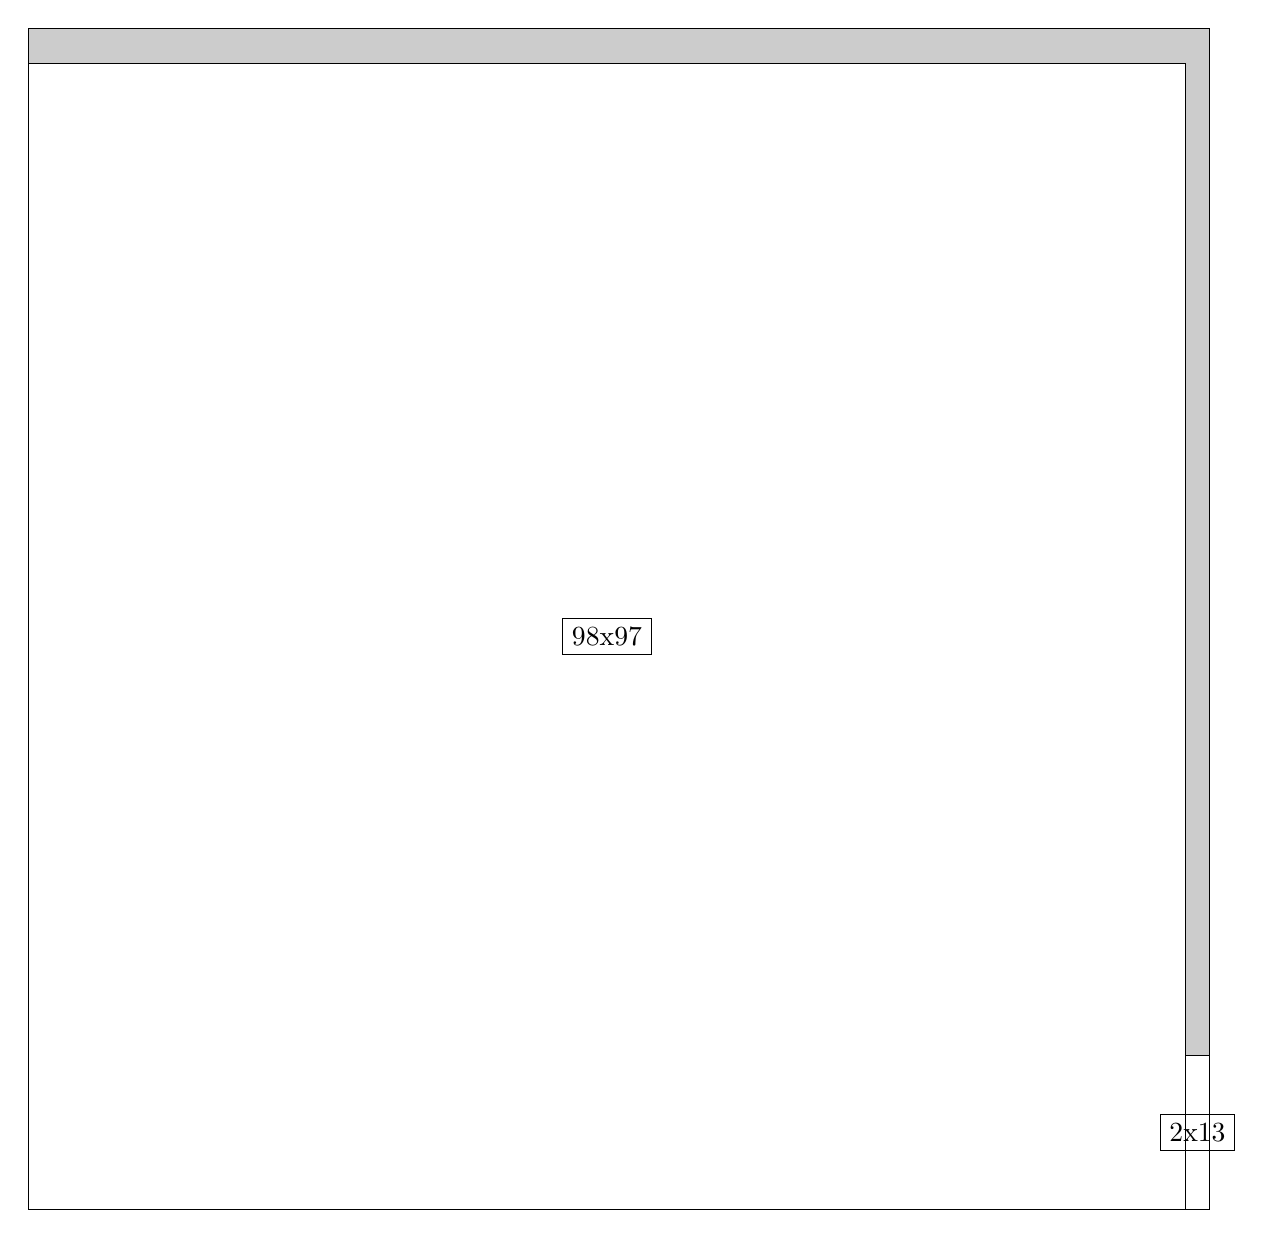
\begin{tikzpicture}[shorten >=1pt,scale=1.0,every node/.style={scale=1.0},->]
\tikzstyle{vertex}=[circle,fill=black!25,minimum size=14pt,inner sep=0pt]
\filldraw[fill=gray!40!white, draw=black] (0,0) rectangle (15.0,15.0);
\foreach \name/\x/\y/\w/\h in {98x97/0.0/0.0/14.7/14.549999999999999,2x13/14.7/0.0/0.3/1.95}
\filldraw[fill=white!40!white, draw=black] (\x,\y) rectangle node[draw] (\name) {\name} ++(\w,\h);
\end{tikzpicture}


w =98 , h =97 , x =0 , y =0 , v =9506
\par
w =2 , h =13 , x =98 , y =0 , v =26
\par
\newpage


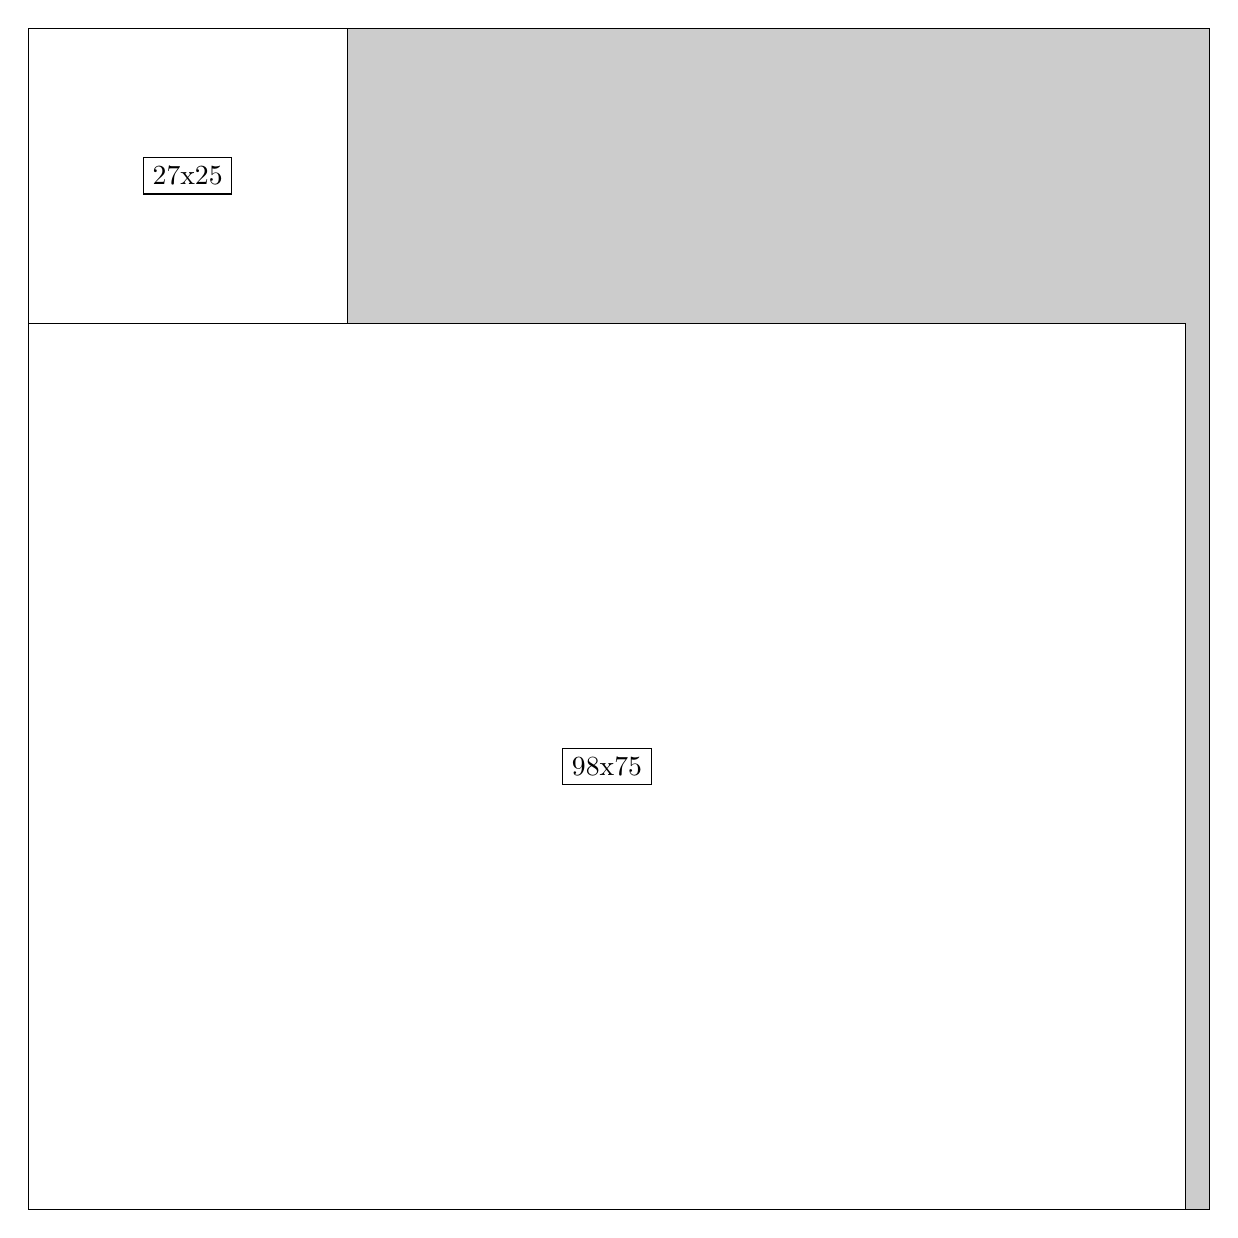
\begin{tikzpicture}[shorten >=1pt,scale=1.0,every node/.style={scale=1.0},->]
\tikzstyle{vertex}=[circle,fill=black!25,minimum size=14pt,inner sep=0pt]
\filldraw[fill=gray!40!white, draw=black] (0,0) rectangle (15.0,15.0);
\foreach \name/\x/\y/\w/\h in {98x75/0.0/0.0/14.7/11.25,27x25/0.0/11.25/4.05/3.75}
\filldraw[fill=white!40!white, draw=black] (\x,\y) rectangle node[draw] (\name) {\name} ++(\w,\h);
\end{tikzpicture}


w =98 , h =75 , x =0 , y =0 , v =7350
\par
w =27 , h =25 , x =0 , y =75 , v =675
\par
\newpage


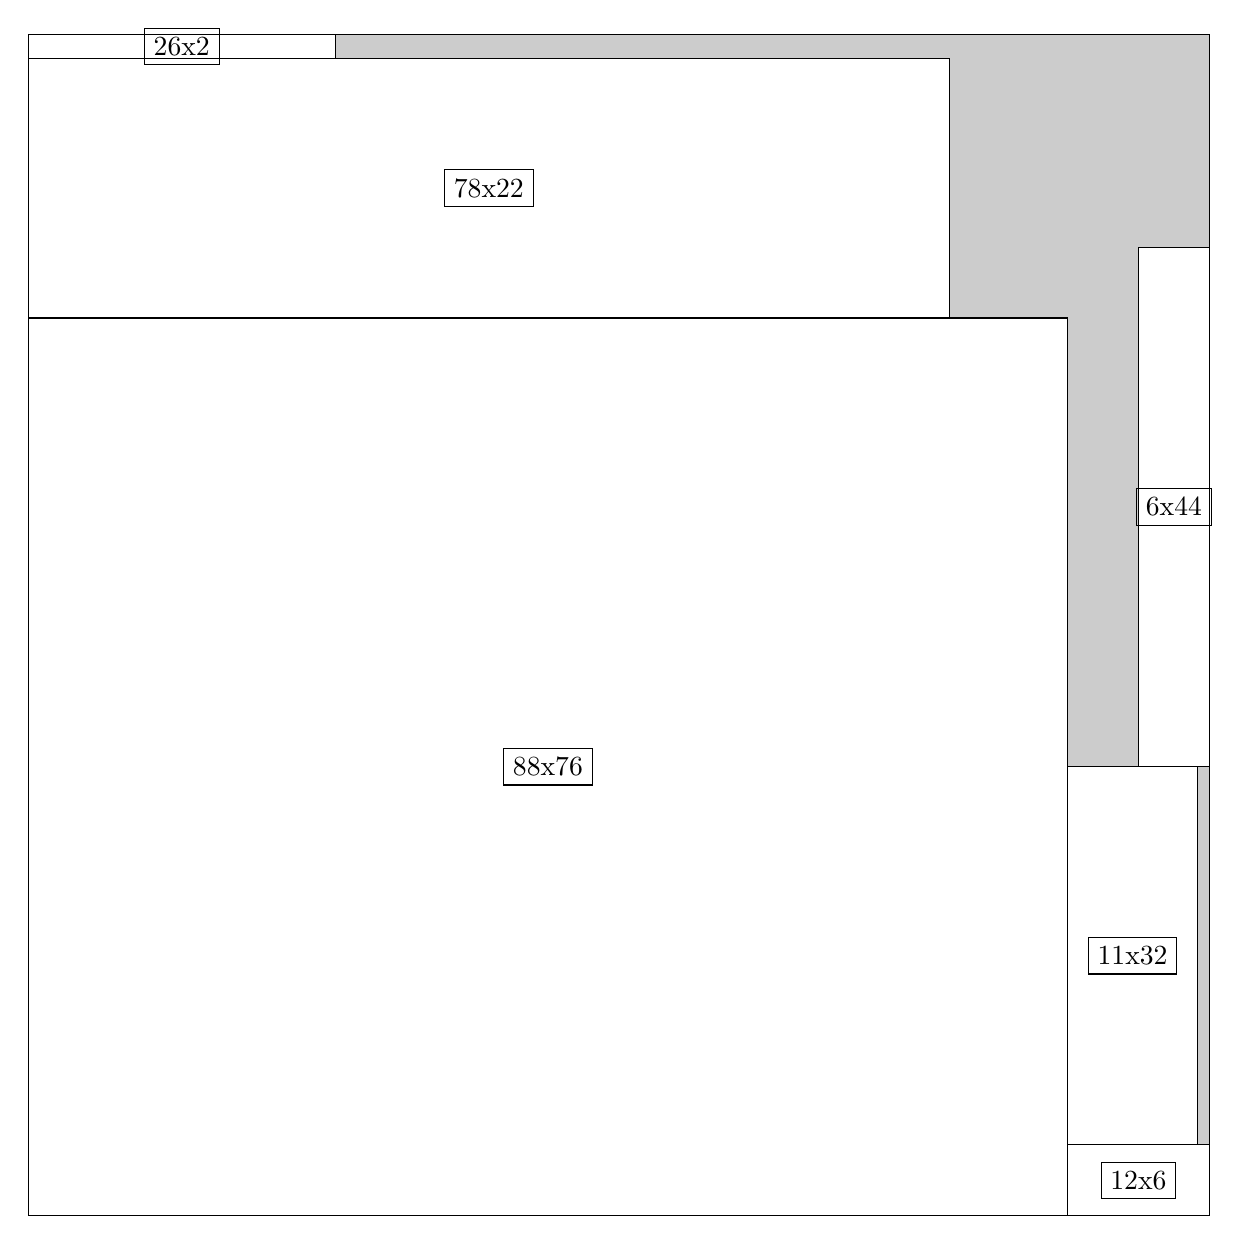
\begin{tikzpicture}[shorten >=1pt,scale=1.0,every node/.style={scale=1.0},->]
\tikzstyle{vertex}=[circle,fill=black!25,minimum size=14pt,inner sep=0pt]
\filldraw[fill=gray!40!white, draw=black] (0,0) rectangle (15.0,15.0);
\foreach \name/\x/\y/\w/\h in {88x76/0.0/0.0/13.2/11.4,78x22/0.0/11.4/11.7/3.3,11x32/13.2/0.8999999999999999/1.65/4.8,6x44/14.1/5.7/0.8999999999999999/6.6,12x6/13.2/0.0/1.7999999999999998/0.8999999999999999,26x2/0.0/14.7/3.9/0.3}
\filldraw[fill=white!40!white, draw=black] (\x,\y) rectangle node[draw] (\name) {\name} ++(\w,\h);
\end{tikzpicture}


w =88 , h =76 , x =0 , y =0 , v =6688
\par
w =78 , h =22 , x =0 , y =76 , v =1716
\par
w =11 , h =32 , x =88 , y =6 , v =352
\par
w =6 , h =44 , x =94 , y =38 , v =264
\par
w =12 , h =6 , x =88 , y =0 , v =72
\par
w =26 , h =2 , x =0 , y =98 , v =52
\par
\newpage


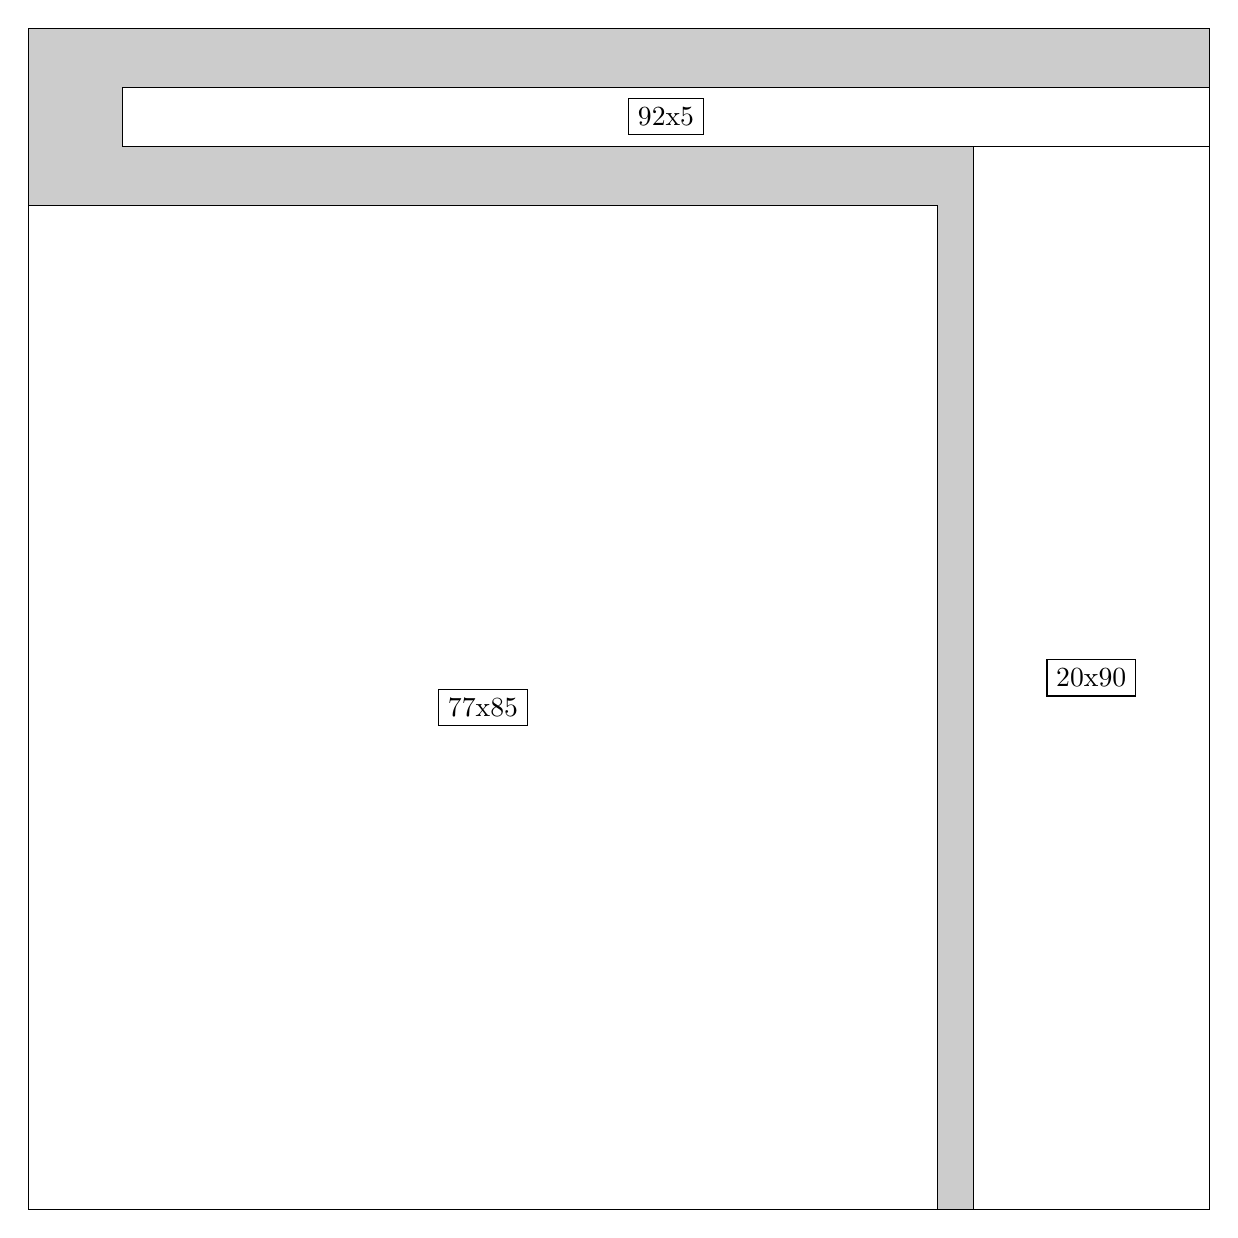
\begin{tikzpicture}[shorten >=1pt,scale=1.0,every node/.style={scale=1.0},->]
\tikzstyle{vertex}=[circle,fill=black!25,minimum size=14pt,inner sep=0pt]
\filldraw[fill=gray!40!white, draw=black] (0,0) rectangle (15.0,15.0);
\foreach \name/\x/\y/\w/\h in {77x85/0.0/0.0/11.549999999999999/12.75,20x90/12.0/0.0/3.0/13.5,92x5/1.2/13.5/13.799999999999999/0.75}
\filldraw[fill=white!40!white, draw=black] (\x,\y) rectangle node[draw] (\name) {\name} ++(\w,\h);
\end{tikzpicture}


w =77 , h =85 , x =0 , y =0 , v =6545
\par
w =20 , h =90 , x =80 , y =0 , v =1800
\par
w =92 , h =5 , x =8 , y =90 , v =460
\par
\newpage


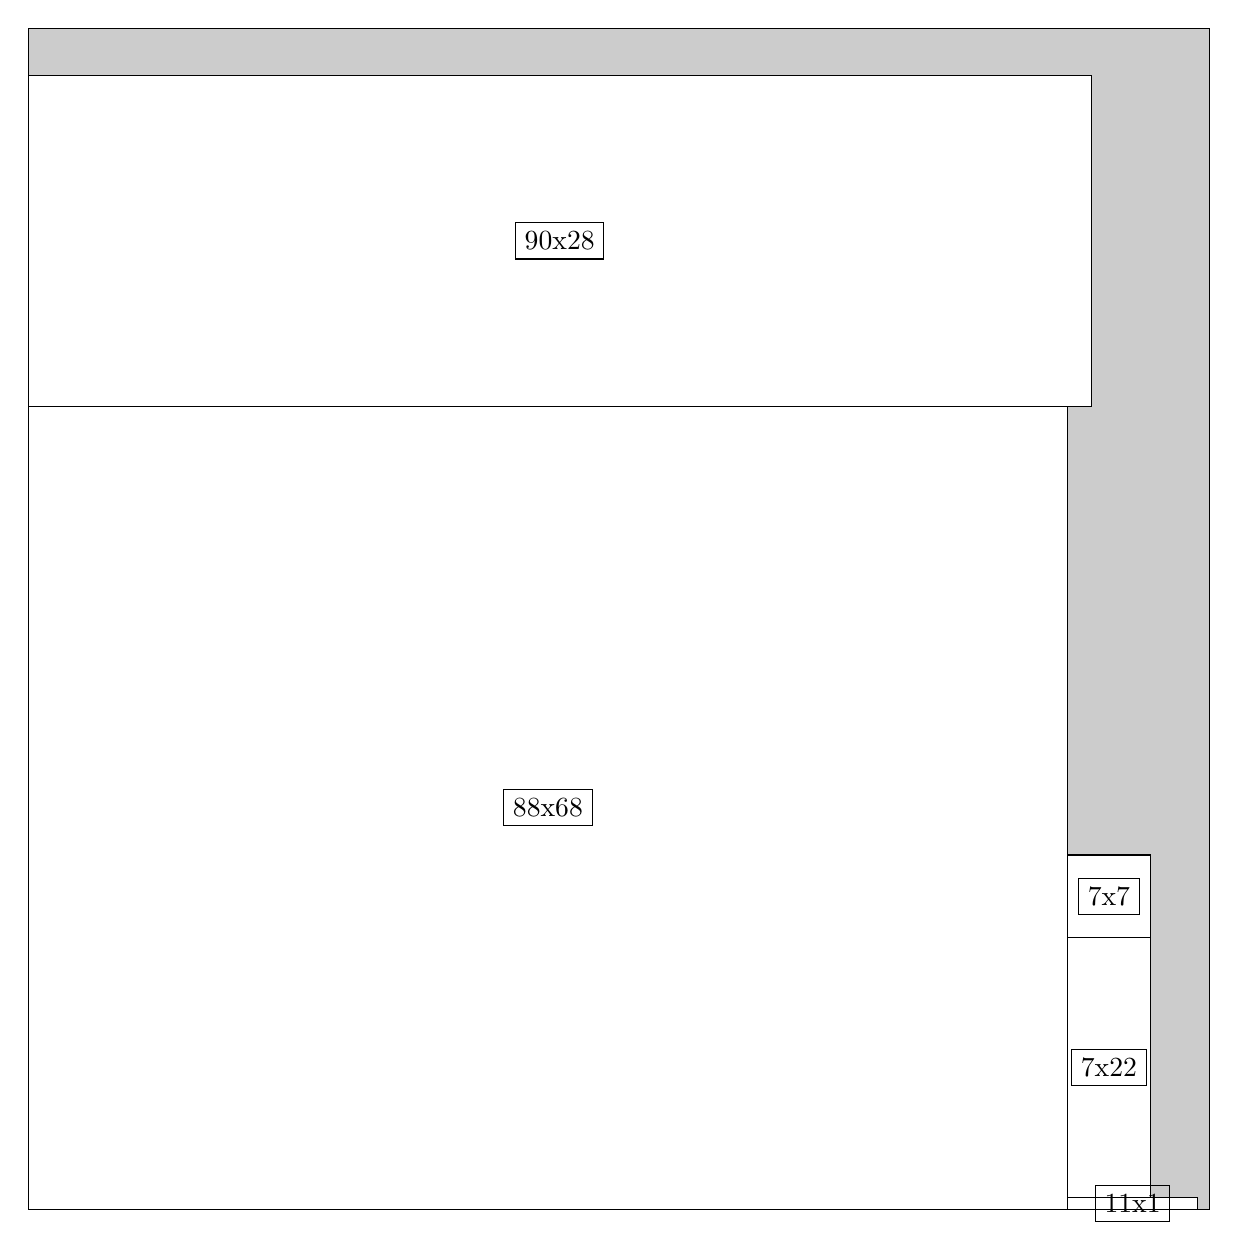
\begin{tikzpicture}[shorten >=1pt,scale=1.0,every node/.style={scale=1.0},->]
\tikzstyle{vertex}=[circle,fill=black!25,minimum size=14pt,inner sep=0pt]
\filldraw[fill=gray!40!white, draw=black] (0,0) rectangle (15.0,15.0);
\foreach \name/\x/\y/\w/\h in {88x68/0.0/0.0/13.2/10.2,90x28/0.0/10.2/13.5/4.2,7x22/13.2/0.15/1.05/3.3,7x7/13.2/3.4499999999999997/1.05/1.05,11x1/13.2/0.0/1.65/0.15}
\filldraw[fill=white!40!white, draw=black] (\x,\y) rectangle node[draw] (\name) {\name} ++(\w,\h);
\end{tikzpicture}


w =88 , h =68 , x =0 , y =0 , v =5984
\par
w =90 , h =28 , x =0 , y =68 , v =2520
\par
w =7 , h =22 , x =88 , y =1 , v =154
\par
w =7 , h =7 , x =88 , y =23 , v =49
\par
w =11 , h =1 , x =88 , y =0 , v =11
\par
\newpage


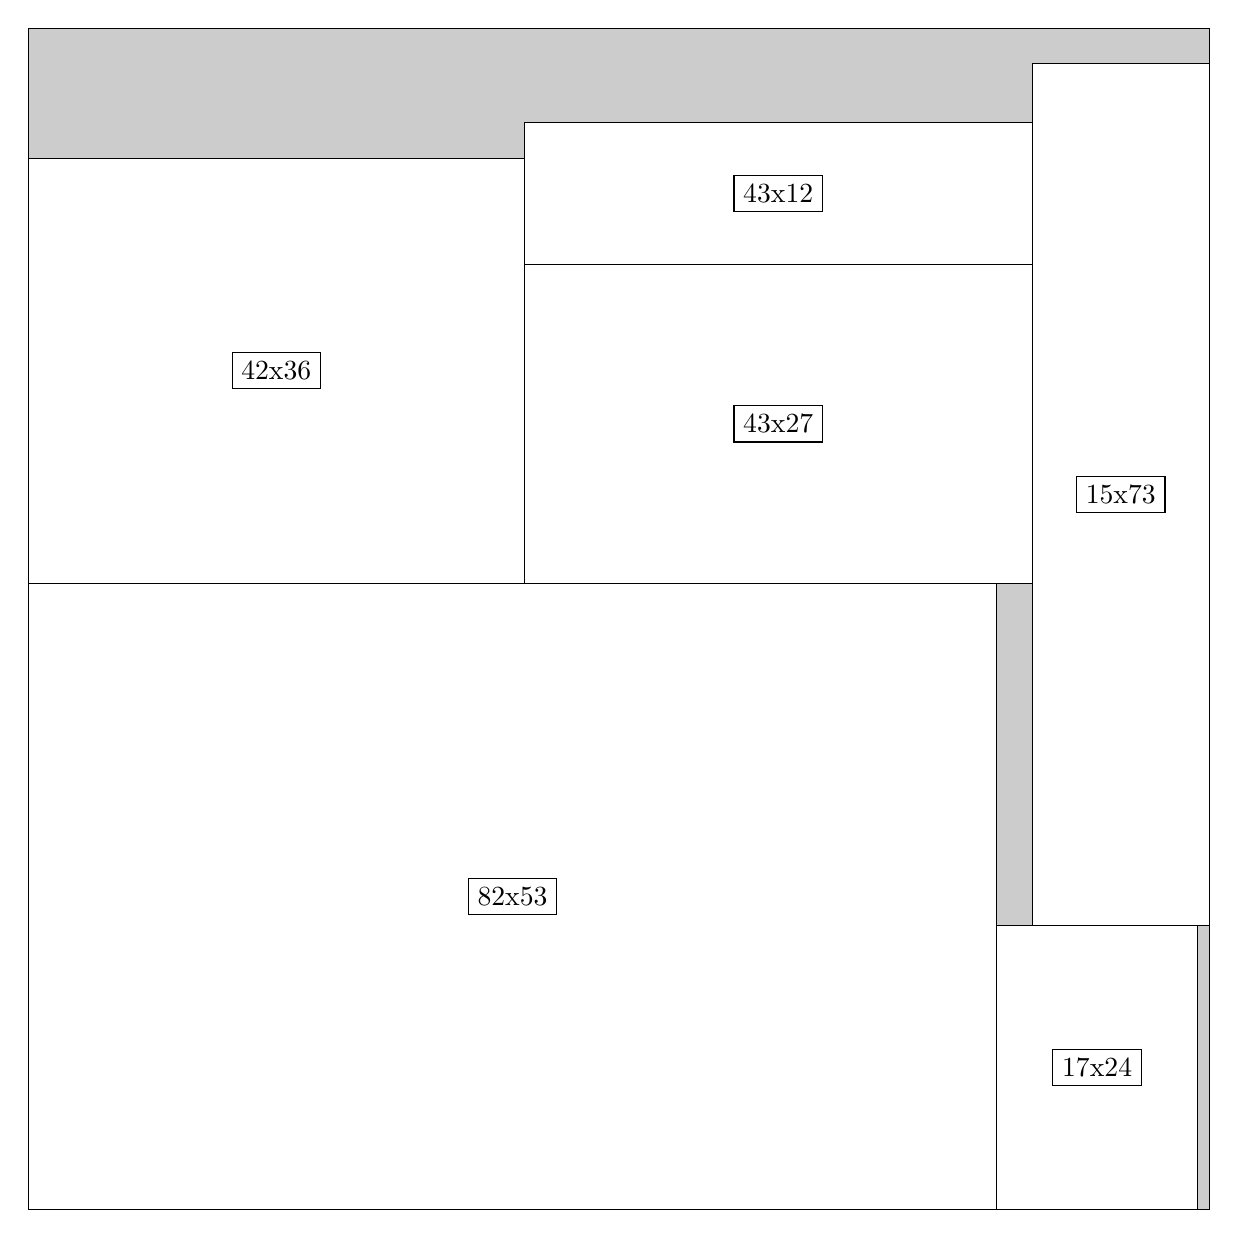
\begin{tikzpicture}[shorten >=1pt,scale=1.0,every node/.style={scale=1.0},->]
\tikzstyle{vertex}=[circle,fill=black!25,minimum size=14pt,inner sep=0pt]
\filldraw[fill=gray!40!white, draw=black] (0,0) rectangle (15.0,15.0);
\foreach \name/\x/\y/\w/\h in {82x53/0.0/0.0/12.299999999999999/7.949999999999999,42x36/0.0/7.949999999999999/6.3/5.3999999999999995,43x27/6.3/7.949999999999999/6.45/4.05,15x73/12.75/3.5999999999999996/2.25/10.95,43x12/6.3/12.0/6.45/1.7999999999999998,17x24/12.299999999999999/0.0/2.55/3.5999999999999996}
\filldraw[fill=white!40!white, draw=black] (\x,\y) rectangle node[draw] (\name) {\name} ++(\w,\h);
\end{tikzpicture}


w =82 , h =53 , x =0 , y =0 , v =4346
\par
w =42 , h =36 , x =0 , y =53 , v =1512
\par
w =43 , h =27 , x =42 , y =53 , v =1161
\par
w =15 , h =73 , x =85 , y =24 , v =1095
\par
w =43 , h =12 , x =42 , y =80 , v =516
\par
w =17 , h =24 , x =82 , y =0 , v =408
\par
\newpage


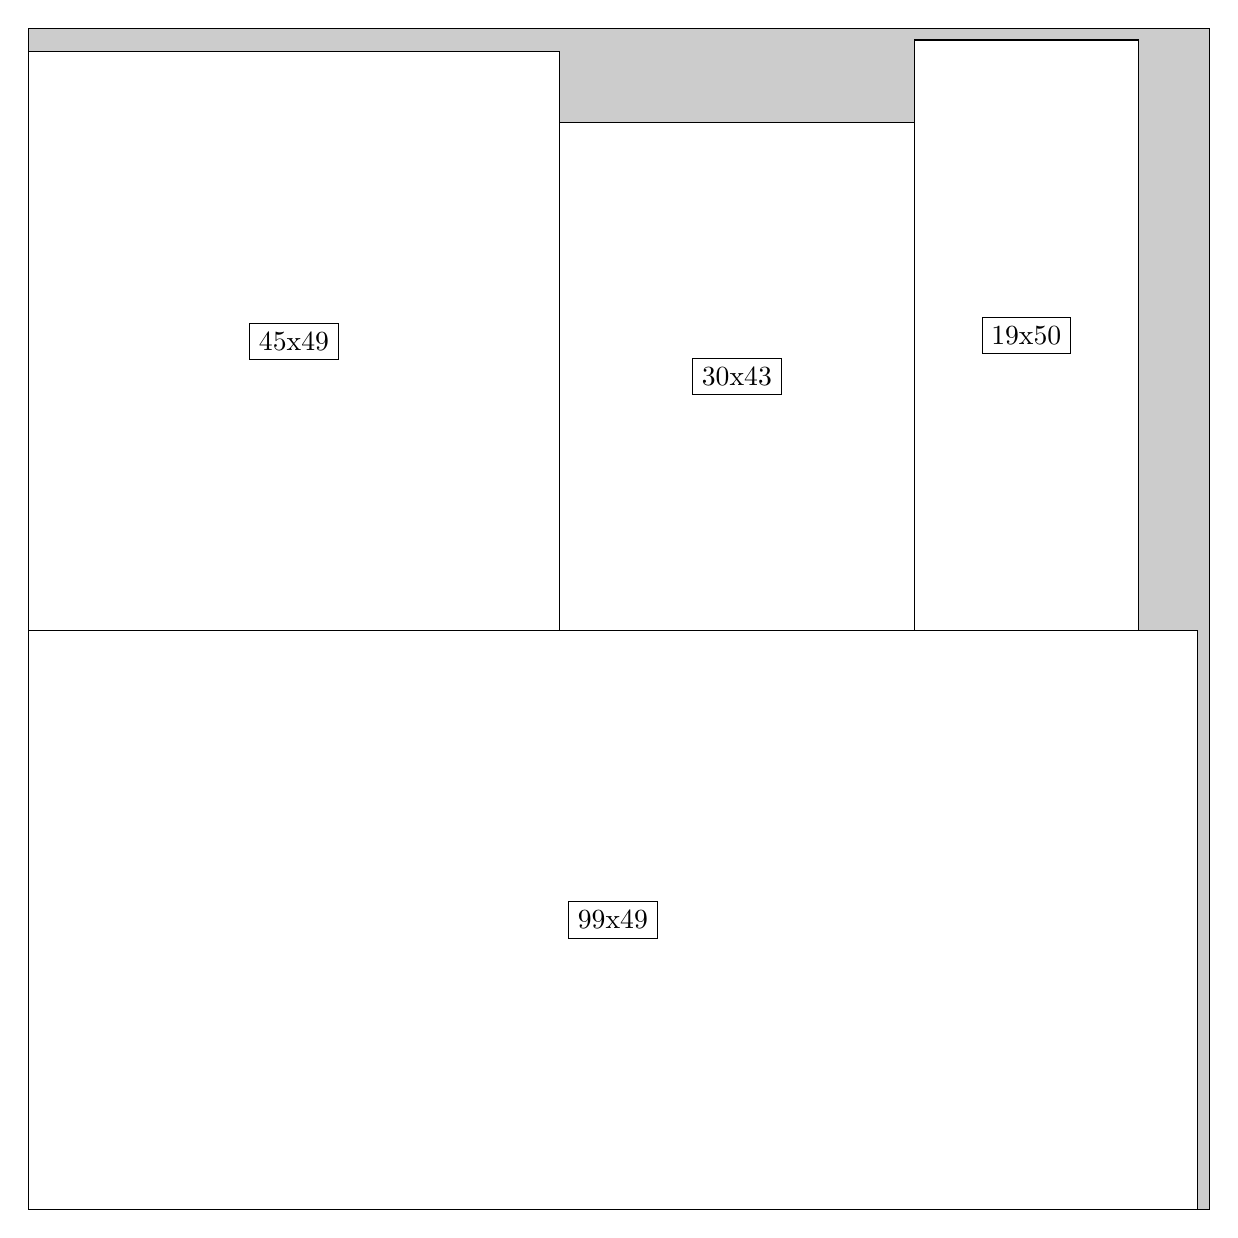
\begin{tikzpicture}[shorten >=1pt,scale=1.0,every node/.style={scale=1.0},->]
\tikzstyle{vertex}=[circle,fill=black!25,minimum size=14pt,inner sep=0pt]
\filldraw[fill=gray!40!white, draw=black] (0,0) rectangle (15.0,15.0);
\foreach \name/\x/\y/\w/\h in {99x49/0.0/0.0/14.85/7.35,45x49/0.0/7.35/6.75/7.35,30x43/6.75/7.35/4.5/6.45,19x50/11.25/7.35/2.85/7.5}
\filldraw[fill=white!40!white, draw=black] (\x,\y) rectangle node[draw] (\name) {\name} ++(\w,\h);
\end{tikzpicture}


w =99 , h =49 , x =0 , y =0 , v =4851
\par
w =45 , h =49 , x =0 , y =49 , v =2205
\par
w =30 , h =43 , x =45 , y =49 , v =1290
\par
w =19 , h =50 , x =75 , y =49 , v =950
\par
\newpage


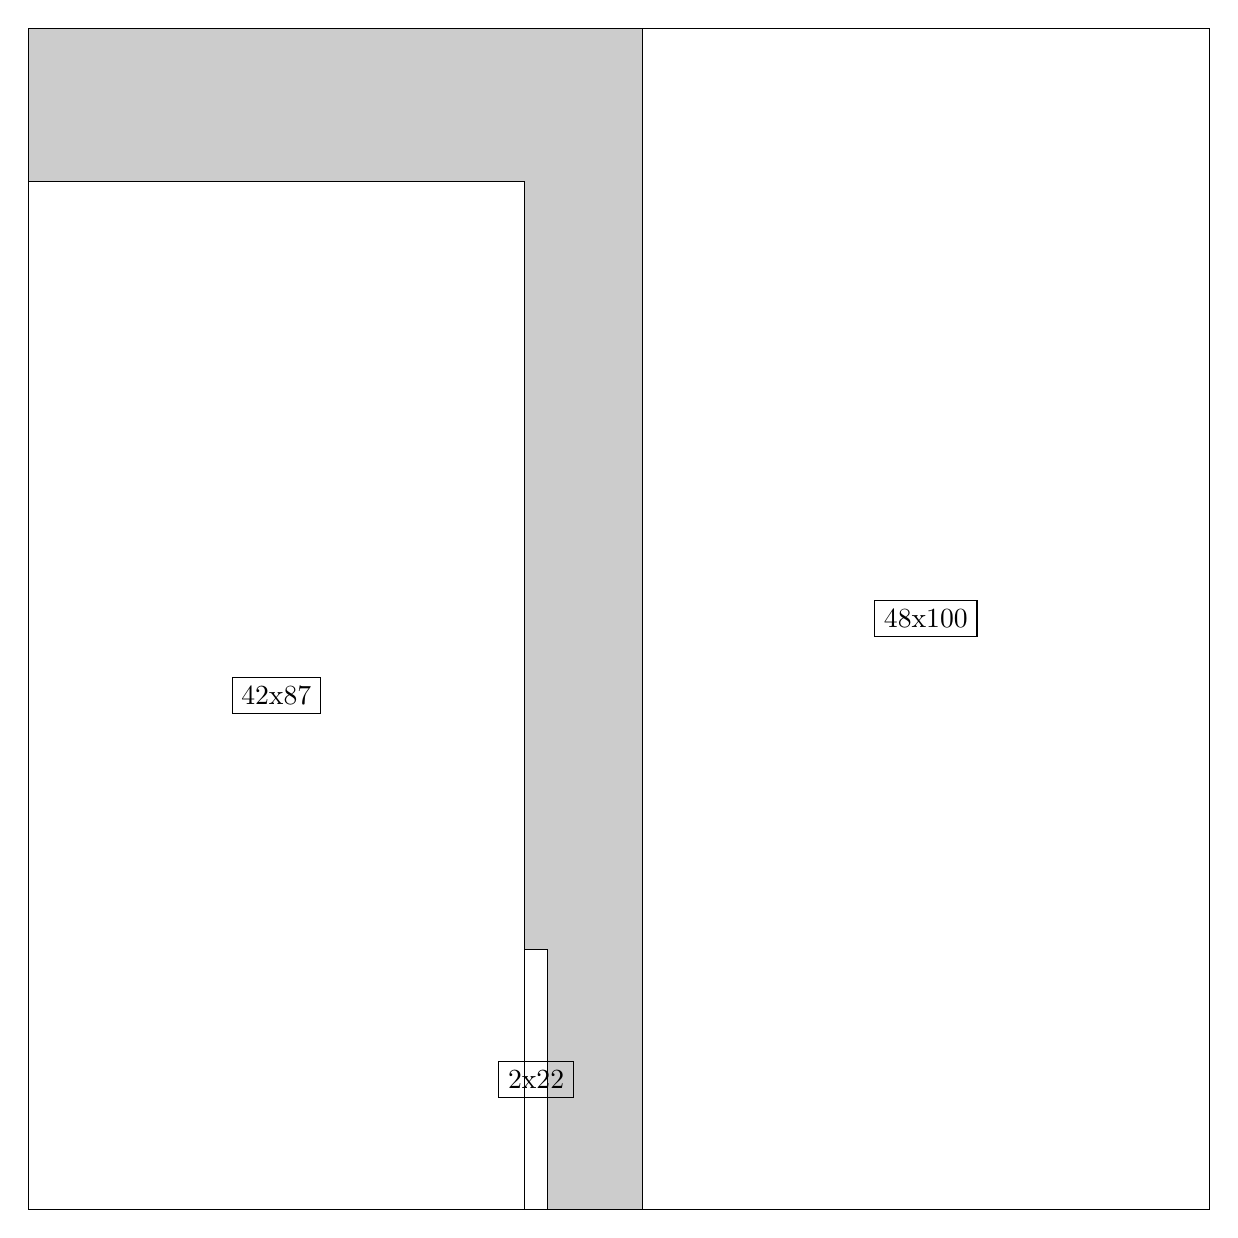
\begin{tikzpicture}[shorten >=1pt,scale=1.0,every node/.style={scale=1.0},->]
\tikzstyle{vertex}=[circle,fill=black!25,minimum size=14pt,inner sep=0pt]
\filldraw[fill=gray!40!white, draw=black] (0,0) rectangle (15.0,15.0);
\foreach \name/\x/\y/\w/\h in {48x100/7.8/0.0/7.199999999999999/15.0,42x87/0.0/0.0/6.3/13.049999999999999,2x22/6.3/0.0/0.3/3.3}
\filldraw[fill=white!40!white, draw=black] (\x,\y) rectangle node[draw] (\name) {\name} ++(\w,\h);
\end{tikzpicture}


w =48 , h =100 , x =52 , y =0 , v =4800
\par
w =42 , h =87 , x =0 , y =0 , v =3654
\par
w =2 , h =22 , x =42 , y =0 , v =44
\par
\newpage


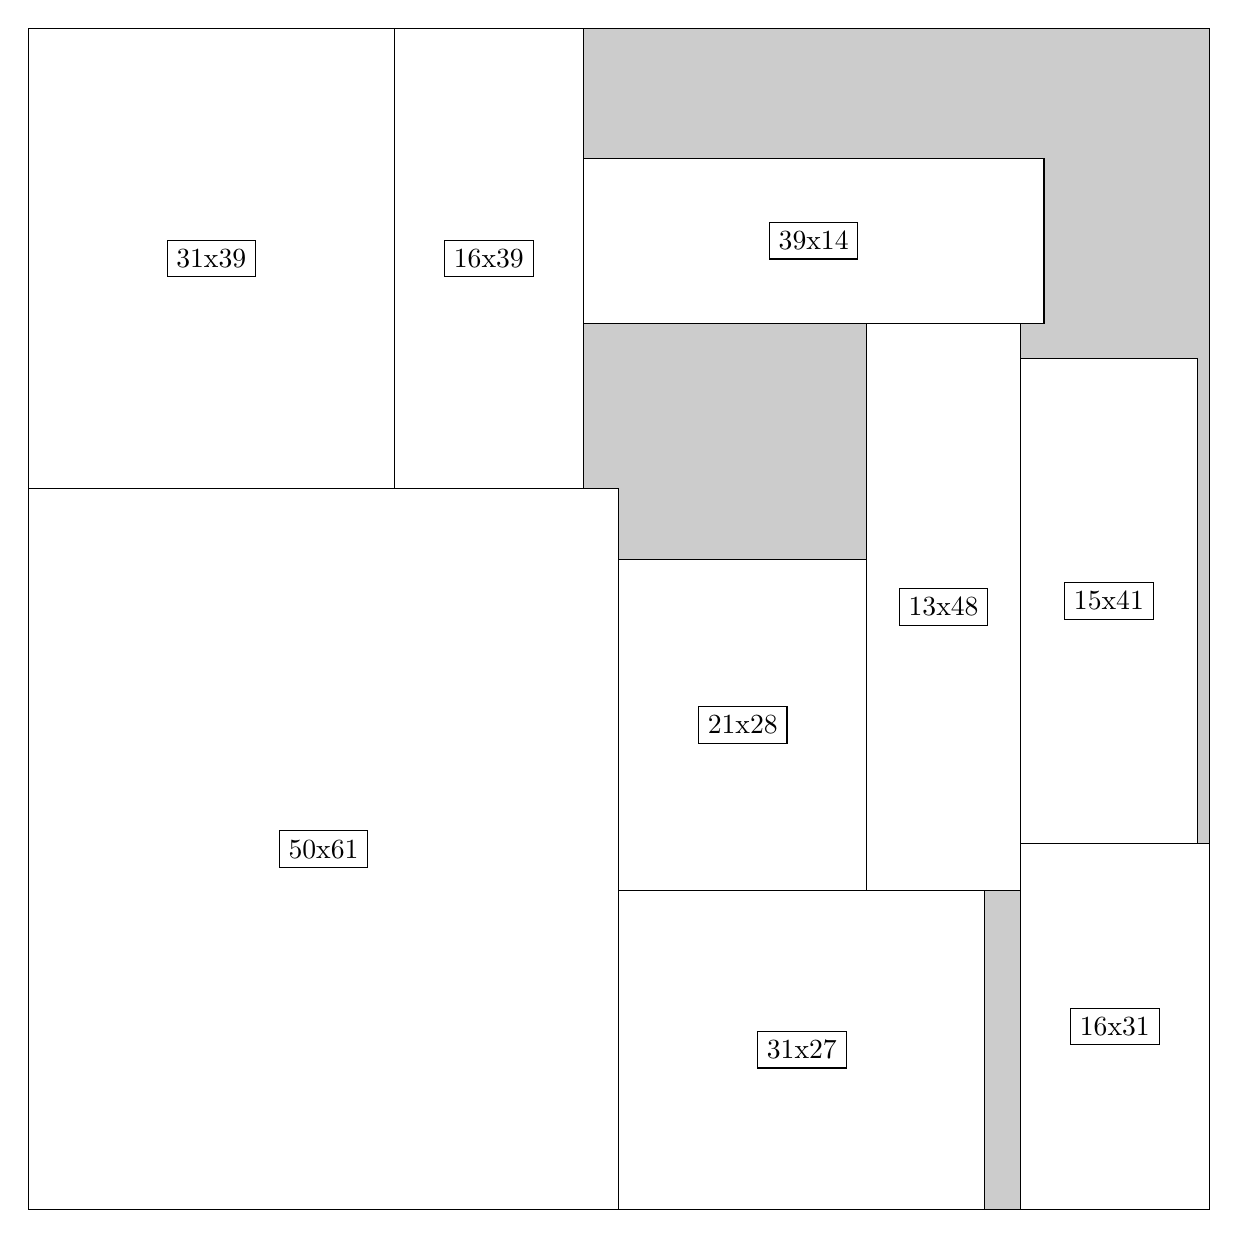
\begin{tikzpicture}[shorten >=1pt,scale=1.0,every node/.style={scale=1.0},->]
\tikzstyle{vertex}=[circle,fill=black!25,minimum size=14pt,inner sep=0pt]
\filldraw[fill=gray!40!white, draw=black] (0,0) rectangle (15.0,15.0);
\foreach \name/\x/\y/\w/\h in {50x61/0.0/0.0/7.5/9.15,31x39/0.0/9.15/4.6499999999999995/5.85,31x27/7.5/0.0/4.6499999999999995/4.05,21x28/7.5/4.05/3.15/4.2,13x48/10.65/4.05/1.95/7.199999999999999,15x41/12.6/4.6499999999999995/2.25/6.1499999999999995,16x39/4.6499999999999995/9.15/2.4/5.85,39x14/7.05/11.25/5.85/2.1,16x31/12.6/0.0/2.4/4.6499999999999995}
\filldraw[fill=white!40!white, draw=black] (\x,\y) rectangle node[draw] (\name) {\name} ++(\w,\h);
\end{tikzpicture}


w =50 , h =61 , x =0 , y =0 , v =3050
\par
w =31 , h =39 , x =0 , y =61 , v =1209
\par
w =31 , h =27 , x =50 , y =0 , v =837
\par
w =21 , h =28 , x =50 , y =27 , v =588
\par
w =13 , h =48 , x =71 , y =27 , v =624
\par
w =15 , h =41 , x =84 , y =31 , v =615
\par
w =16 , h =39 , x =31 , y =61 , v =624
\par
w =39 , h =14 , x =47 , y =75 , v =546
\par
w =16 , h =31 , x =84 , y =0 , v =496
\par
\newpage


\end{document}